\chapter{Related Work}\label{related-work}
The work presented in this thesis is based on two main areas of research: the evaluation of Large Language Models (LLMs) and Information Retrieval (IR).
In this chapter, the current state of research in those areas is presented, as it relates to this thesis.
We start with a short introduction to LLMs, then present the current evaluation methods for those models in the field of question answering, since the different versions of question answering tasks, especially long form question answering are most similar to our evaluation setup.

Afterwards, the field of IR is introduced.
Different retrieval methods used in this thesis are presented and why they were chosen for this work.
Additionally, the evaluation metrics used to compare those retrieval methods are introduced.

\section{Evaluation of LLMs for Question Answering}\label{sec:evaluation-of-large-language-models}
Transformer-based language models are generally defined as systems that produce probability distributions over a set of tokens (which can be words, subwords or characters) given the preceding or surrounding context.    
The rise of LLMs started with the introduction of the transformer architecture by \cite{vaswani:2017:Attention}, followed by the release of models like BERT~(\cite{devlin:2018:BERT}) and GPT-2~(\cite{radford:2018:Improving}).
The transformer architecture allowed the models to process more context than previous models, such as LSTM-based methods like ELMo~(\cite{peters:2018:Deep}), or static word embeddings based on statistical co-occurrences like GloVe~(\cite{pennington:2014:Glove}).
This led to improvements in many NLP tasks over earlier methods, as shown by \cite{radford:2018:Improving}, who compare the base GPT performance against multiple then state-of-the-art models on different tasks, improving or performing at least competitively on all of them.

With the release of GPT-3~(\cite{brown:2020:Language}), the size of datasets used to train LLMs, as well as the number of parameters in the models increased significantly.
While GPT-2 in its largest version has a total of 1.5 billion parameters, GPT-3 has 175 billion parameters.
As \cite{wei:2022:Emergent} show, this scale not only leads to improvements over previously used benchmark compared to smaller models, but also to what they call \textit{emergent abilities}.
\textit{Emergent abilities} are abilities that are not present in smaller models.
Those include generating long coherent stories or poems, translating between languages and answering long form questions.
None of those capabilities are present in smaller models, with e.g. the largest version of GPT-2 performing poorly on translation and summarization, as shown in the original paper~(\cite{radford:2018:Improving}).

With the capabilities of LLMs expanding, the task of evaluating them becomes more challenging.

In this section, we focus on the current evaluation methods of Question Answering (QA) capabilities of LLMs and how the task of long form question answering is evaluated.

The field of QA in NLP contains multiple different tasks, which can be grouped into extractive QA, single/multiple choice QA and long form QA.
Those tasks vary in their complexity, with earlier models like BERT and GPT-2 already being benchmarked on extractive QA and single choice QA.

Extractive QA and single/multiple choice QA have in common that they are relatively easy to evaluate.
When evaluating extractive QA the overlap of the predicted tokens with the answer span can be calculated, and for single choice QA the predicted answer option can be compared to the ground truth answer.

This changes when evaluating long form QA.
Here, models are evaluated on their ability to answer questions in a free form manner, without constraining the length of the answer.
Answers can get long and complex, branching out in different directions by including examples or other information.
The evaluation of such answers is not as straightforward as for the other versions of QA, so human evaluation is the gold standard.

In the following, the different QA evaluation tasks are introduced, including popular datasets and evaluation metrics for them.

\subsection{Extractive Question Answering}\label{sec:extractive-qa}
Extractive QA is the task of answering questions given a context containing the answer.
In this context, which can be a short paragraph or entire Wikipedia article, the correct answer span has to be selected by the model.

One of the most popular datasets for evaluating LLMs in this task is SQuAD~(\cite{rajpurkar:2016:SQuAD}), and its successor SQuAD 2.0~(\cite{rajpurkar:2018:Know}), which includes unanswerable questions.
Adding unanswerable questions to the dataset is a way to test the model's ability to detect when a question can not be answered by the given context.
Many other datasets like NarrativeQA~(\cite{kovcisky:2018:The}), QuAC~(\cite{choi:2018:QuAC}) or Natural Questions~(\cite{kwiatkowski:2019:Natural}) are based on the same principle.
They consist of questions written by crowd workers or experts in the field, based on a Wikipedia article snippet or similar text passages.
The exact constraints on the questions and the context vary between the datasets, but the general idea is the same.
Figure~\ref{fig:extractive_qa_example} shows a generic example of a question from an extractive QA dataset.
\begin{figure}[tb]
    \centering
    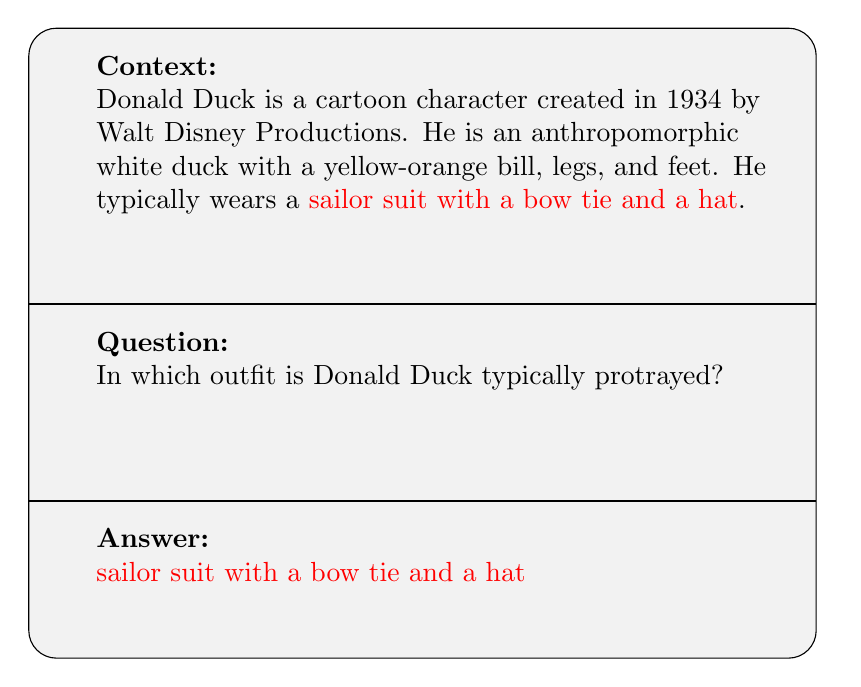
\begin{tikzpicture}
        % Draw paper background
        \draw[fill=gray!10,rounded corners=1em] (0,0) rectangle (10,8);
        % Draw text
        \node[align=left,anchor=north west, text width=9cm,inner sep=1em] at (0.5,8.0) {
            \textbf{Context:}

            Donald Duck is a cartoon character created in 1934 by Walt Disney Productions. He is an anthropomorphic white duck with a yellow-orange bill, legs, and feet. He typically wears a \textcolor{red}{sailor suit with a bow tie and a hat}.
        };
        % Draw vertical line
        \draw[thick] (0,4.5) -- (10,4.5);
        % Draw question
        \node[align=left,anchor=north west, text width=9cm,inner sep=1em] at (0.5,4.5) {
            \textbf{Question:}

            In which outfit is Donald Duck typically protrayed?
        };
        % Draw vertical line
        \draw[thick] (0,2.0) -- (10,2.0);
        % Draw question
        \node[align=left,anchor=north west, text width=9cm,inner sep=1em] at (0.5,2.0) {
            \textbf{Answer:}

            \textcolor{red}{sailor suit with a bow tie and a hat}
        };
    \end{tikzpicture}
    \caption{Example of a typical extractive question answering task: The answer span ``sailor suit with a bow tie and a hat'' is highlighted in red in the paragraph.}
    \label{fig:extractive_qa_example}
\end{figure}

The evaluation metrics for tasks of this category are based on the overlap between the predicted answer span and the ground truth answer span.
Specifically, this would be the exact match (EM) score, which measures the percentage of exact matches between the predicted and the ground truth answer span.
Alternatively, the F1 score as the harmonic mean of precision and recall can be used, with precision being defined as
\[ \text{precision} = \frac{\text{number of correct tokens in prediction}}{\text{total number of tokens in the prediction}} \]
and recall as
\[ \text{recall} = \frac{\text{number of correct tokens in prediction}}{\text{total number of tokens in the ground truth}} \]
with a correct token being a predicted token that overlaps with the ground truth answer.
The F1 score is then calculated as
\[ \text{F1} = 2 \times \frac{\text{precision} \times \text{recall}}{\text{precision} + \text{recall}} \]
which is the harmonic mean of precision and recall.

Earlier LLMs like BERT have to be specifically fine-tuned for the task of extractive QA.
For each token in the provided context, the model assigns a probability of the token being the starting or ending token of the answer span~(\cite{devlin:2018:BERT}).

Later models like GPT-3 are able to directly generate the answer from the context and the questions without any fine-tuning, by using the zero-shot, single-shot or multi-shot capabilities of the model~(\cite{brown:2020:Language}).
In some settings of the datasets, the context can be completely omitted, forcing the model to directly answer the question.
This means that the results of the two approaches are not directly comparable, because even though the models were evaluated on the same dataset, the approaches are fundamentally different.

\subsection{Single and Multiple Choice Question Answering}\label{sec:multiple-choice-qa}
For single and multiple choice question answering, the model has to select the correct answer from a set of possible answers, which can be done with or without context.
While most datasets are single choice datasets, some datasets (like MultiRC by \cite{khashabi:2018:Looking}) are multiple choice, so that the model has to check each answer for correctness, instead of just selecting the best fitting one.
Questions for single and multiple choice QA often stem from official exams, like the MMLU dataset~(\cite{hendrycks:2020:Measuring}), which combines question from many exams like the United States Medical Licensing Examination or the Examination for Professional Practice in Psychology.
In other datasets, the questions are collected from crowd workers and verified by experts~(\cite{clark:2018:Think},~\cite{mihaylov:2018:Can}).

\begin{figure}[tb]
    \centering
    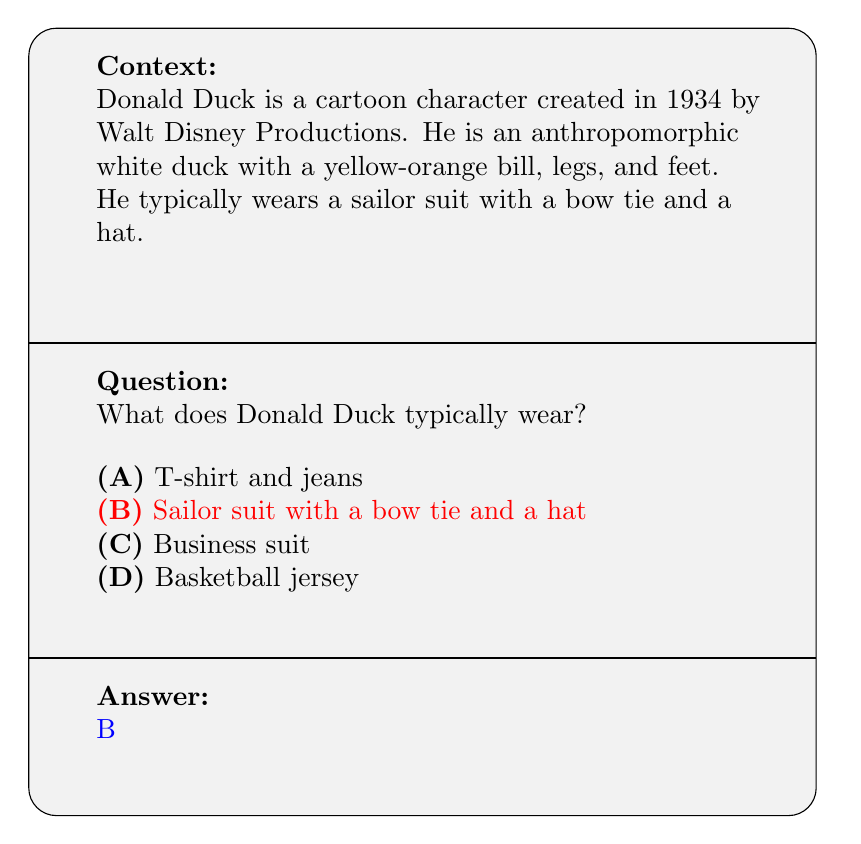
\begin{tikzpicture}
        % Draw paper background
        \draw[fill=gray!10,rounded corners=1em] (0,0) rectangle (10,10);
        % Draw text
        \node[align=left,anchor=north west, text width=8.5cm,inner sep=1em] at (0.5,10.0) {
            \textbf{Context:}

            Donald Duck is a cartoon character created in 1934 by Walt Disney Productions. He is an anthropomorphic white duck with a yellow-orange bill, legs, and feet. He typically wears a sailor suit with a bow tie and a hat.
        };
        % Draw vertical line
        \draw[thick] (0,6) -- (10,6);
        % Draw question
        \node[align=left,anchor=north west, text width=8.5cm,inner sep=1em] at (0.5,6) {
            \textbf{Question:}

            What does Donald Duck typically wear?
        };
        % Draw multiple-choice options
        \node[align=left,anchor=north west, text width=8.5cm,inner sep=1em] at (0.5,4.8) {
            \textbf{(A)} T-shirt and jeans

            \textcolor{red}{\textbf{(B)} Sailor suit with a bow tie and a hat}

            \textbf{(C)} Business suit

            \textbf{(D)} Basketball jersey
        };
        \draw[thick] (0,2) -- (10,2);
        \node[align=left,anchor=north west, text width=9cm,inner sep=1em] at (0.5,2) {
            \textbf{Answer:}

            \textcolor{blue}{B}
        };
    \end{tikzpicture}
    \caption{Example of a single choice question with context: The correct option is highlighted in red.
    The blue B would be a possible answer generated by the LLM, after being primed with the context and the question.
    }\label{fig:mc_example}
\end{figure}
Figure \ref{fig:mc_example} shows an example of a single choice question with context.
The LLM is provided with the context, the question and the answer options and a ``Answer: '' prefix.
Based on this, the model has to select one of the given options.

Evaluation is straightforward in this case, the model's generated answer option is compared to the ground truth answer and accuracy over all questions is calculated.

\subsection{Long Form Question Answering}\label{sec:long-form-qa}
\begin{figure}[tb]
    \centering
    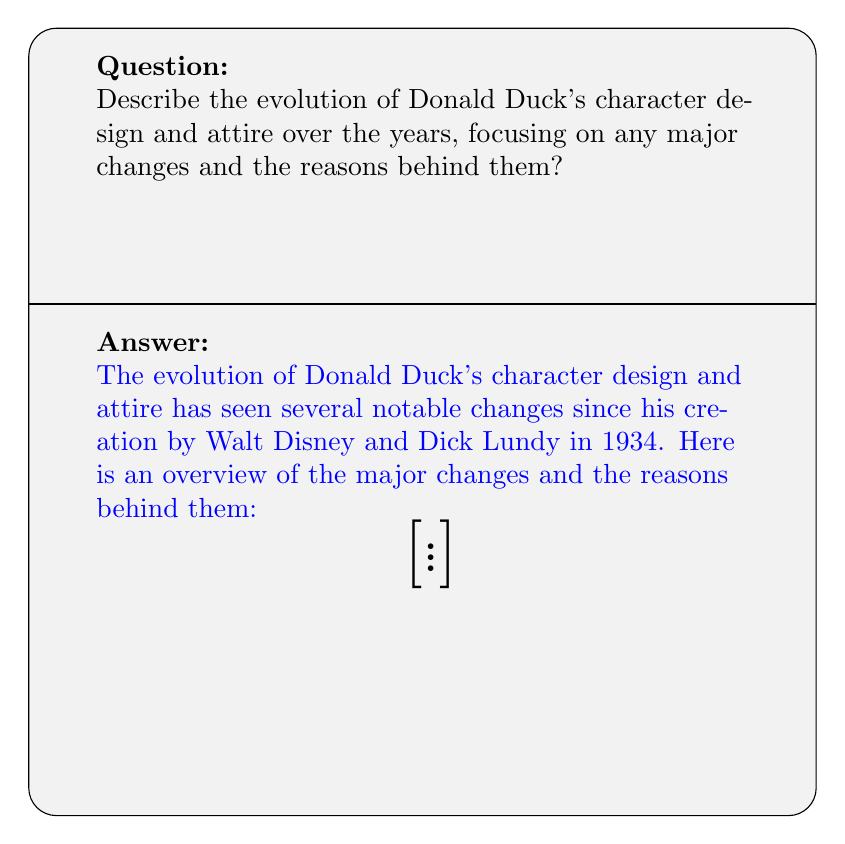
\begin{tikzpicture}
        % Draw paper background for question
        \draw[fill=gray!10,rounded corners=1em] (0,0) rectangle (10,10);
        % Draw question
        \node[align=left,anchor=north west, text width=8.5cm,inner sep=1em] at (0.5,10) {
            \textbf{Question:}

            Describe the evolution of Donald Duck's character design and attire over the years, focusing on any major changes and the reasons behind them?
        };
        % Draw vertical line
        \draw[thick] (0,6.5) -- (10,6.5);
        % Draw sample answer
        \node[align=left,anchor=north west, text width=8.5cm,inner sep=1em] at (0.5,6.5) {
            \textbf{Answer:}

            \textcolor{blue}{The evolution of Donald Duck's character design and attire has seen several notable changes since his creation by Walt Disney and Dick Lundy in 1934. Here is an overview of the major changes and the reasons behind them:}
            

            \centerline{\Huge [\vdots]}
        };
    \end{tikzpicture}
    \caption{Example of Long-Form QA without Context: The question prompts for a detailed answer about Donald Duck's character evolution and attire. The prompt given to the model is written in black, the sample answer (generated by ChatGPT-3.5) is written in blue. The generated answer continues for multiple paragraphs.}
    \label{fig:long_form_qa_example_with_answer}
\end{figure}
Long form QA refers to the task of answering open-ended questions, which can usually not be answered by simply providing one entity or number, but require an in-depth answer.
% Similar tasks exist in the IR community, e.g. generating query biased summaries as described by \cite{tombros:1998}, in which a retrieval model retrieves and summarizes documents given a user query.
With LLMs being deployed in chatbots and as such expected to deliver answers mostly without context, evaluating the models on long form QA is important.

So far, only a handful of datasets are available for this task, with the first dataset in this category being the ELI5 dataset~(\cite{fan:2019:ELI5}).
It consists of questions and the corresponding highest voted answer from the "Explain Like I'm Five" subreddit, where users ask questions about complex topics, which are then answered by other users.
They are accompanied by support documents, which are retrieved from web sources by querying for the original question.
This dataset was used to by~\cite{nakano:2021:Webgpt} to fine-tune GPT-3 for the task of long form QA without using the context documents.
The answers given by the fine-tuned model are evaluated by humans, by comparing them to the highest voted answer from the ELI5 dataset.

An additional dataset for this task is the MultiMedQA~(\cite{singhal:2023:Towards}), which curates questions from multiple other datasets used previously. 
Answers generated by physicians are used as ground truth answers.
Those are then compared to the model generated answers by other physicians, as well as by laypeople.
Additionally, the answers were individually rated in different rubrics, introduced in a previous work~(\cite{singhal:2022:Large}).

None of the papers for current, main-stream LLMs like GPT-3~(\cite{brown:2020:Language}), GPT-4~(\cite{openai:2023:GPT}) or Llama 2~(\cite{touvron:2023:Llama}) include evaluations on common benchmarks for this category.
This shows that long form QA is still a relatively new task, lacking sufficient academic benchmarks.

\subsection{Difficulties of Long Form Question Answering}\label{sec:long-form-qa-difficulties}
Recent works have shown multiple challenges in the task of long form question answering, independently of which model architecture is used to answer the questions.
Since the answers are free form text, and not just a multiple choice option, one number or one entity, the quality of the model can't be measured using accuracy or similar metrics that require static ground truth information.
Multiple evaluation dimensions are of interest, for example:
\begin{itemize}
    \item \textbf{Relevance:} Are the most important aspects of the query answered?
    \item \textbf{Readability:} How easy is the answer to read and understand?
    \item \textbf{Credibility:} Are there any references provided and are they of high quality?
\end{itemize}
This adds additional complexity to the evaluation process, compared to other QA tasks which only measure correctness of the answer.


\cite{xu:2023:A} focus on the evaluation process of LFQA, comparing different automatic evaluation methods to human judgement.
They differentiate between general-purpose generation evaluation metrics, which were originally designed for other NLP tasks like summarization or translation, and fine-tuned metrics, which are fine-tuned to LFQA.
The following types of metrics are considered general-purpose metrics, used in the same way in different NLP tasks:
\begin{itemize}
\item \textbf{Answer-reference metrics:} Include metrics like ROUGE or BERTScore. These metrics compare generated answers to reference answers, focusing on aspects like lexical overlap and semantic similarity.
\item \textbf{Answer-only metrics:} Such as Self-BLEU which measure the fluency and diversity of generated text. These are intrinsic metrics of the generated text and do not need a reference answer for evaluation.
\item \textbf{Question-answer metrics:} Score answers given the question in one of two ways: either by calculating the likelihood of questions given an answer, or by using an encoder model to score sequences given a prefix.
\item \textbf{Answer-evidence metrics:} Judge the given answer by the evidence documents used to generate it. This method indirectly assesses the answer's credibility and factual accuracy.
\end{itemize}
In addition to these metrics, \cite{xu:2023:A} evaluate two different versions of fine-tuned metrics.
The first one is based on Longformer~(\cite{beltagy:2020:Longformer}), in which the model is fine-tuned to produce a score given a question and an answer, optionally combined with evidence documents.
The second model is a fine-tuned version of GPT-3, which is trained to output either \emph{Answer1} or \emph{Answer2} given a question and two answer options.
Both fine-tuned models are trained on the dataset generated by \cite{nakano:2021:Webgpt}, which contains human preference labels for different answer pairs.

All automatic evaluation methods are evaluated on the task of choosing the preferable answer given two long form answers to a question.
The results are compared to previous human judgement on the same task.
They find that one of their baseline models, choosing always the longest answer, performs almost as good as the fine-tuned GPT-3 model, which outperformed all other methods.
Both variants are still outperformed by human annotations, which is the gold standard.

\cite{krishna:2021:Hurdles} investigates in more detail the problems of reference based evaluation metrics like ROUGE-L. 
They highlight that those metrics are unable to capture answer components like examples if those examples are not present in the ground truth answers. 

Furthermore, they note that even human evaluation is limited in judging long form QA over different models.
Some problems include the hiring process of experts, especially when datasets tackle multiple fields of expertise.
Finding experts of similar education and background is challenging when doing evaluations of different models over a span of time.
Additionally, the evaluation process is more mentally challenging for the individual annotator the longer the answers get.
Similar problems have previously been shown by \cite{akoury:2020:Storium} in the context of machine generated stories.
They find that crowd workers have low agreement for different evaluation metrics when evaluating the same stories.
They tackle this problem by using gamification techniques to activate online users of a story writing platform to evaluate and improve the generated stories.
A similar approach is taken by \cite{dugan:2020:RoFT}, who implement a website where users try to differentiate machine-generated text from human generated text.

This shows that there are still many obstacles to overcome in the task of evaluating long form QA systems.
We try to tackle some of those problems with the approach presented in this thesis.
To incorporate multiple metrics, we first compare and evaluate multiple retrieval methods on the previously mentioned metrics of relevance, readability and credibility.
This ensures that the document ranking is optimized for multiple dimensions, instead of just one.
Based on the findings by \cite{xu:2023:A} how shows that of the automated metrics the transformer-based models perform best, we compare multiple transformer-based model for the retrieval step.

Since our approach of tackling this problem uses concepts from the field of information retrieval, a short overview of relevant methods is given in the next section.

%------------------------------------------------------------------
%------------------------------------------------------------------
%------------------------------------------------------------------

\section{Retrieval Models}\label{sec:retrieval-models}
Since we want to use retrieval methods to evaluate the performance of LLMs, we will give some background on the field of Information Retrieval(IR), and how it relates to long form QA.
IR is the process of retrieving relevant information based on an information need, from a collection of documents, usually in the form of whole documents, passages or single sentences.
A brief overview of a retrieval pipeline based on ``An introduction to information retrieval'' by \cite{manning:2009:An} is provided now.

In most IR systems, the document corpus first has to be brought into a form that is more suitable for retrieval.
This process usually starts with a step to reduce to total size of the vocabulary, using tokenization, stemming, stop word removal and other techniques.
This removes unnecessary information from the documents, which would otherwise increase the size of the index, which is created in the next step.
Commonly, this is an inverted index, which maps each term in the corpus to the documents that contain it.
Now, given a query, an IR system returns a ranked list of documents that are most relevant to the query.
To achieve this, IR systems estimate a relevance score for each document in the collection with respect to the query.
The documents are then ranked according to their relevance scores, with the most relevant documents appearing at the top of the list.
Some pipelines include a re-ranking step, in which the most relevant documents are re-ranked after the first retrieval using a more expensive (and hopefully more effective) retrieval model.
Figure \ref{fig:reranking_pipeline} shows a basic retrieval pipeline, in which the re-ranking step is optional.
\begin{figure}[tb]
\centering
\begin{tikzpicture}[node distance=0.8cm, auto]

% Styles for boxes
\tikzstyle{box} = [rectangle, draw, fill=blue!10, text width=4.5em, text centered, rounded corners, minimum height=3em]
\tikzstyle{user} = [ellipse, draw, fill=blue!30, text width=4.5em, text centered, rounded corners, minimum height=3em]

% Nodes
\node [box, fill=blue!30] (corpus) {Document Corpus};
\node [box, fill=blue!30, right=of corpus] (index) {Index};
\node [box, fill=blue!30, right=of index] (model) {Retrieval Model};
\node [user, above=of model] (query) {Queries};
\node [box, fill=blue!5, right=of model] (rerank) {Re-ranking};
\node [box, fill=blue!30, right=of rerank] (output) {Ranked Documents};

% Edges
\draw[->] (corpus) -- (index);
\draw[->] (query) -- (model);
\draw[->] (index) -- (model);
\draw[->] (model) -- (rerank);
\draw[->] (rerank) -- (output);

\end{tikzpicture}
\caption{Depiction of a basic retrieval pipeline, with optional re-ranking step. The process begins with a document corpus, which is indexed to facilitate efficient retrieval. Given the information need of a user in the form of a query, the retrieval model returns the most relevant documents. Optionally, the documents can be re-ranked using a re-ranking model which is usually more resource intensive.}
\label{fig:reranking_pipeline}
\end{figure}

\subsection{Baseline Retrieval Models}\label{sec:baseline-retrieval-models}
First, we will look at the basic retrieval models, which are used as baselines in this thesis.
They have been chosen because they were shown to be effective on the used dataset in previous work~(\cite{goeuriot:2021:Consumer}).
Both models use the implementation in the Terrier IR platform~(\cite{ounis:2005:Terrier}).

\subsubsection{TF-IDF}\label{sec:tf-idf}
Term Frequency-Inverse Document Frequency (tf-idf) is one of the most commonly used models in information retrieval.
It measures the importance of a term in a document relative to a collection of documents or corpus.
The central intuition is that terms that appear frequently in a document but not in many other documents in the corpus are significant and thus should be given higher weight.

Given a query \( q \) consisting of terms \( t_1,t_2,\cdots,t_n \) and a document corpus \( D \) of size \( N \) we calculate the score of \( q \) given document \( d \) by first calculating the tf-idf of each term  in \( q \) given \( d \) and then summing them up.
\[ \text{tf-idf}(t, d) = \text{tf}(t, d) \times \text{idf}(t) \]
Where \( \text{tf}(t, d) \) is the frequency of term \( t \) in document \( d \) and 
\[ \text{idf}(t) = \log \left( \frac{N}{1 + \text{df}(t)} \right) \]
where document frequency \( \text{df}(t) \) is the number of documents containing term \( t \).
The final score of the query given the document is then calculated as
\[ \text{score}(q, d) = \sum_{t \in q} \text{tf-idf}(t, d) \]
For retrieval given a query \( q \) tf-idf scores are calculated for all documents, which are then ranked according to their score.

In the Terrier IR platform, the implementation of tf-idf uses variants of the tf and idf components.
For Term Frequency, the Robertson's tf formulation~(\cite{robertson:2004:Understanding}) is used, which incorporates an additional parameter that adds a saturation effect to the term frequency.
For idf, the original formulation by Sparck Jones~(\cite{sparck:1972:A}) is applied.

\subsubsection{DPH}\label{sec:dph}
Divergence from Randomness (DFR) is a framework in IR that assigns term weights based on the divergence of the actual within-document term frequency distribution from a random term frequency distribution~(\cite{amati:2006:Frequentist}).
The divergence from randomness using the hyper-geometric distribution model(DPH) is one of the models derived from the DFR framework.

The principle behind DFR is that terms that are informative in a document will have a distribution that deviates significantly from what would be expected if terms were distributed randomly.
While TF-IDF emphasizes the importance of terms based on their frequency in a document and their inverse frequency in the corpus, DPH focuses on the divergence of a term's distribution from what would be expected under a random distribution.
Specifically, DPH assesses the divergence using the hyper-geometric distribution.
In essence, where TF-IDF weights terms based on their prominence and rarity, DPH weights them based on how much their occurrence pattern deviates from randomness.
The implementation in the Terrier IR platform follows the original formulation by \cite{amati:2006:Frequentist}.


\subsection{Transformer-based Retrieval Models}\label{sec:transformer-retrieval-models}
As mentioned in earlier sections, transformer-based models have been shown to be effective on a variety of tasks, including IR.
There are different approaches of how transformers can be used for retrieval, a brief overview of methods used in this thesis is given here.
All transformer models are a form of learning-to-rank, in which the model is trained on a dataset to predict which documents are relevant to a query.
This differentiates them from our baseline models, which rule-based and do not require training.

Two of the most common transformer based architectures are cross-encoder and bi-encoder models.
\begin{figure}[tb]
  \centering
  % Define colors
  \definecolor{textcolor}{RGB}{255, 230, 204}
  \definecolor{encodercolor}{RGB}{204, 229, 255}
  \definecolor{embeddingcolor}{RGB}{217, 234, 211}
  \definecolor{scorecolor}{RGB}{230, 204, 255} % New color for scores

  % Bi-Encoder
  \begin{minipage}{.48\textwidth}
    \centering
    \begin{tikzpicture}[node distance=0.7cm, auto, every node/.style={scale=0.8}]
      \tikzstyle{text_in} = [rectangle, rounded corners, minimum width=3cm, minimum height=1cm, align=center, draw=black, fill=textcolor]
      \tikzstyle{encoder} = [rectangle, rounded corners, minimum width=3cm, minimum height=1cm, align=center, draw=black, fill=encodercolor]
      \tikzstyle{embedding} = [rectangle, rounded corners, minimum width=3cm, minimum height=1cm, align=center, draw=black, fill=embeddingcolor]
      \tikzstyle{score} = [ellipse, minimum width=2cm, minimum height=1cm, align=center, draw=black, fill=scorecolor]

      % Nodes
      \node[text_in] (query) {Query};
      \node[encoder, below=of query] (qencoder) {Query Encoder};
      \node[embedding, below=of qencoder] (qembed) {Query Embedding};
      
      \node[text_in, right=of query, xshift=1cm] (doc) {Document};
      \node[encoder, below=of doc] (docencoder) {Doc Encoder};
      \node[embedding, below=of docencoder] (docembed) {Doc Embedding};

      \node[score, below=of qembed.south, xshift=2.5cm] (biScore) {Relevance Score}; % New node for relevance score

      % Arrows
      \draw[-{Latex[length=3mm]}] (query) -- (qencoder);
      \draw[-{Latex[length=3mm]}] (qencoder) -- (qembed);
      \draw[-{Latex[length=3mm]}] (qembed) -- (biScore);
      \draw[-{Latex[length=3mm]}] (doc) -- (docencoder);
      \draw[-{Latex[length=3mm]}] (docencoder) -- (docembed);
      \draw[-{Latex[length=3mm]}] (docembed) -- (biScore);

    \end{tikzpicture}
    \caption{Bi-Encoder Architecture. Query and document are encoded separately, then the relevance is calculated based on similarity measures between the embeddings.}
    \label{fig:bi-encoder}
  \end{minipage}
  \hfill
  % Cross-Encoder
  \begin{minipage}{.48\textwidth}
    \centering
    \begin{tikzpicture}[node distance=0.7cm, auto, every node/.style={scale=0.8}]
      \tikzstyle{text_in} = [rectangle, rounded corners, minimum width=3cm, minimum height=1cm, align=center, draw=black, fill=textcolor]
      \tikzstyle{encoder} = [rectangle, rounded corners, minimum width=3cm, minimum height=1cm, align=center, draw=black, fill=encodercolor]
      \tikzstyle{embedding} = [rectangle, rounded corners, minimum width=3cm, minimum height=1cm, align=center, draw=black, fill=embeddingcolor]
      \tikzstyle{score} = [ellipse, minimum width=2cm, minimum height=1cm, align=center, draw=black, fill=scorecolor]

      % Nodes
      \node[text_in, right=] (query) {Query};

      \node[text_in, right=of query, xshift=1cm] (doc) {Document};

      \node[text_in, below=of query.south, xshift=2.5cm] (qdoc) {Query $+$ Document};

      \node[encoder, below=of qdoc] (qencoder) {Cross-Encoder};

      \node[score, below=of qencoder] (biScore) {Relevance Score};
      % Arrows
      \draw[-{Latex[length=3mm]}] (query) -- (qdoc);
      \draw[-{Latex[length=3mm]}]  (doc) -- (qdoc);
      \draw[-{Latex[length=3mm]}] (qdoc) -- (qencoder);
      \draw[-{Latex[length=3mm]}] (qencoder) -- (biScore);

    \end{tikzpicture}
    \caption{Cross-Encoder Architecture. Query and document are first combined and then fed to the Cross-Encoder, the relevance is directly calculated by the encoder.}
    \label{fig:cross-encoder}
  \end{minipage}
\end{figure}
Bi-encoders independently embed queries and documents using transformer models like BERT~(\cite{devlin:2018:BERT}) or T5~(\cite{roberts:2019:Exploring}).
For the document collection, this can be done offline since the embeddings are independent of the query.
This separation allows them to efficiently process large datasets as the embeddings can be pre-computed and stored.
It also enables rapid retrieval, since at inference time only the embedding for the current query has to be calculated and compared to the pre-computed document embeddings.
The documents are then ranked according to their embedding similarity to the query.

Cross-encoders, on the other hand, take a combined input sequence of both query and document and produce a scalar relevance score.
This joint modeling enables them to better capture the interaction and nuances between a query and a document.
Due to their fine-grained interaction modeling, cross-encoders outperform bi-encoders in terms of precision in retrieving relevant documents as shown by \cite{thakur:2020:Augmented} and \cite{rosa:2022:In}.
However, the need to process each query-document pair individually makes them computationally demanding, especially for large datasets.
As a result, they are typically only used in second-stage retrieval, where the objective is to re-rank the top results obtained from an initial retrieval method.

The following sections describe the different transformer-based retrieval models used in this thesis.
\subsubsection{MonoT5 + DuoT5}\label{sec:monot5-duot5}
MonoT5 and DuoT5~(\cite{roberts:2019:Exploring}), are based on previous work by \cite{nogueira:2019:Multi}, who introduced monoBERT and duoBERT, first applying transformer architecture to the task of document ranking.
The general idea is to first use a baseline retrieval model like BM25 to retrieve an initial set of relevant documents.
Then, pairs of the query and each document in the initial set are concatenated and fed into the mono version of the transformer model, which produces a scalar score for each query-document pair.
The documents with the highest scores are then fed into the duo model, which takes the query and each possible pair of documents as input, outputting a probability of one document being more relevant than the other.
Given those scores, the documents are re-ranked another time, serving as the final output of the retrieval pipeline.
The main difference between the BERT and T5 versions, is that for BERT the [CLS] token from embedding the query and the document can be used as input to a single layer neural network, to output a probability of the document being relevant.
Since there is no [CLS] token for models in the T5 family, as they are sequence-to-sequence model, this part is done using an input template:
\begin{equation}
    \text{Query: \emph{q} Document: \emph{d} Relevant:}
\end{equation} 
where the model is fine-tuned to produce the token \emph{true} or \emph{false} given query \emph{q} and document \emph{d}.

At inference, softmax is applied to the \emph{true} and \emph{false} tokens only, the scores are then calculated using the probability of the \emph{true} token.
This works analogously for the Duo version of both models, by just adding the second document.
MonoT5 and DuoT5 both belong to the family of cross-encoder models, sharing the general characteristics of those models.

This model architecture allows for precisely tuning retrieval efficiency vs. effectiveness, by parameterizing how many documents are filtered in each step, making the model suitable for different usecases.


\subsubsection{ColBERT}\label{sec:colbert}
\begin{figure}[tb]
\centering
% Define colors
\definecolor{textcolor}{RGB}{255, 230, 204}
\definecolor{encodercolor}{RGB}{204, 229, 255}
\definecolor{embeddingcolor}{RGB}{217, 234, 211}
\definecolor{similaritycolor}{RGB}{255, 204, 204} % New color for similarity scores
\definecolor{scorecolor}{RGB}{230, 204, 255} % New color for scores
% ColBERT Retrieval Model
\begin{tikzpicture}[node distance=0.7cm, auto, every node/.style={scale=0.8}]
\tikzstyle{text_in} = [rectangle, rounded corners, minimum width=3cm, minimum height=1cm, align=center, draw=black, fill=textcolor]
\tikzstyle{token} = [rectangle, rounded corners, minimum width=0.5cm, minimum height=1cm, align=center, draw=black, fill=textcolor]
\tikzstyle{encoder} = [rectangle, rounded corners, minimum width=3cm, minimum height=1cm, align=center, draw=black, fill=encodercolor]
\tikzstyle{embedding} = [rectangle, rounded corners, minimum width=0.5cm, minimum height=1cm, align=center, draw=black, fill=embeddingcolor]
\tikzstyle{similarity} = [ellipse, minimum width=1cm, minimum height=1cm, align=center, draw=black, fill=similaritycolor]
\tikzstyle{score} = [ellipse, minimum width=2cm, minimum height=1cm, align=center, draw=black, fill=scorecolor]
% black thick dotted border around document, doc encoder and doc embeddings
\tikzstyle{highlight}= [draw=black, rounded corners, inner sep=1cm, dashed, thick]

\node[text_in] (query) {Query};
\node[token, below=of query, xshift=-1cm] (q1) {};
\node[token, below=of query] (q2) {};
\node[token, below=of query, xshift=1cm] (q3) {};
\node[encoder, below=of q2] (qencoder) {Query Encoder};
\node[embedding, below=of qencoder, xshift=-1cm] (qe1) {};
\node[embedding, below=of qencoder] (qe2) {};
\node[embedding, below=of qencoder, xshift=1cm] (qe3) {};

\node[text_in, right=of query, xshift=3cm] (doc) {Document};
\node[token, below=of doc, xshift=-1cm] (d1) {};
\node[token, below=of doc] (d2) {};
\node[token, below=of doc, xshift=1cm] (d3) {};
\node[encoder, below=of d2] (docencoder) {Doc Encoder};
\node[embedding, below=of docencoder, xshift=-1cm] (de1) {};
\node[embedding, below=of docencoder] (de2) {};
\node[embedding, below=of docencoder, xshift=1cm] (de3) {};

\node[similarity, below=of qe2.south] (maxSim1) {MaxSim};
\node[similarity, below=of qe2.south, xshift=3.5cm] (maxSim2) {MaxSim};
\node[similarity, below=of de2.south] (maxSim3) {MaxSim};

\node[score, below=of maxSim2] (score1) {Sum};

% draw highlight box around document, doc encoder and doc embeddings. Label above the box says "Offline"
\node[highlight, fit=(doc) (docencoder) (de1) (de2) (de3), label={[align=center]above:Offline}] (docbox) {};

% Arrows
\draw[-{Latex[length=3mm]}] ([xshift=-0.8cm]query.south) -- (q1.north);
\draw[-{Latex[length=3mm]}] (query.south) -- (q2.north);
\draw[-{Latex[length=3mm]}] ([xshift=0.8cm]query.south) -- (q3.north);
\draw[-{Latex[length=3mm]}] (q1.south) -- ([xshift=-0.8cm]qencoder.north);
\draw[-{Latex[length=3mm]}] (q2.south) -- (qencoder.north);
\draw[-{Latex[length=3mm]}] (q3.south) -- ([xshift=0.8cm]qencoder.north);
\draw[-{Latex[length=3mm]}] ([xshift=-0.8cm]qencoder.south) -- (qe1.north);
\draw[-{Latex[length=3mm]}] (qencoder.south) -- (qe2.north);
\draw[-{Latex[length=3mm]}] ([xshift=0.8cm]qencoder.south) -- (qe3.north);
\draw[-{Latex[length=3mm]}] ([xshift=-0.8cm]doc.south) -- (d1.north);
\draw[-{Latex[length=3mm]}] (doc.south) -- (d2.north);
\draw[-{Latex[length=3mm]}] ([xshift=0.8cm]doc.south) -- (d3.north);
\draw[-{Latex[length=3mm]}] (d1.south) -- ([xshift=-0.8cm]docencoder.north);
\draw[-{Latex[length=3mm]}] (d2.south) -- (docencoder.north);
\draw[-{Latex[length=3mm]}] (d3.south) -- ([xshift=0.8cm]docencoder.north);
\draw[-{Latex[length=3mm]}] ([xshift=-0.8cm]docencoder.south) -- (de1.north);
\draw[-{Latex[length=3mm]}] (docencoder.south) -- (de2.north);
\draw[-{Latex[length=3mm]}] ([xshift=0.8cm]docencoder.south) -- (de3.north);
% draw dotted arrows from query and document to maxSim1, maxSim2 and maxSim3
\draw[-{Latex[length=3mm]}] (qe1.south) -- (maxSim1);
\draw[-{Latex[length=3mm]}] (qe2.south) -- (maxSim2);
\draw[-{Latex[length=3mm]}] (qe3.south) -- (maxSim3);
\draw[-{Latex[length=3mm]}, dashed] (de1.south) -- (maxSim1);
\draw[-{Latex[length=3mm]}, dashed] (de1.south) -- (maxSim2);
\draw[-{Latex[length=3mm]}, dashed] (de1.south) -- (maxSim3);
\draw[-{Latex[length=3mm]}, dashed] (de2.south) -- (maxSim1);
\draw[-{Latex[length=3mm]}, dashed] (de2.south) -- (maxSim2);
\draw[-{Latex[length=3mm]}, dashed] (de2.south) -- (maxSim3);
\draw[-{Latex[length=3mm]}, dashed] (de3.south) -- (maxSim1);
\draw[-{Latex[length=3mm]}, dashed] (de3.south) -- (maxSim2);
\draw[-{Latex[length=3mm]}, dashed] (de3.south) -- (maxSim3);
\draw[-{Latex[length=3mm]}] (maxSim1.south) -- (score1);
\draw[-{Latex[length=3mm]}] (maxSim2.south) -- (score1);
\draw[-{Latex[length=3mm]}] (maxSim3.south) -- (score1);
\end{tikzpicture}
\caption{ColBERT Retrieval Model. The query and document are processed separately to generate token embeddings. The maximum cosine similarity between all token embeddings of the query and document is calculated and summed over all query tokens, which is the relevance score of the document given the query.}
\label{fig:colbert}
\end{figure}
ColBERT~(\cite{khattab:2020:Colbert}) is another BERT based model for document ranking.
It shares similarities with the general bi-encoder architecture, but introduces some modifications to improve effectiveness.
Instead of representing each document and query as a single vector, ColBERT uses a set of vectors to represent contextualized embeddings for each token in the document or query.
For the documents, this can again be done offline, so that at the retrieval stage, only the embeddings for the query have to be generated and compared to the documents.
The relevance score for document $d$ given query $q$ is estimated using their late interaction model, in which maximum cosine similarity between all query term embeddings and document term embeddings is calculated, and then summed over for all query terms.
This allows for a more fine-grained mapping between query and document terms, also allowing for more fine-grained meaning of different terms.
An efficient computation of the similarity calculation allows ColBERT to scale much better, compared to feeding BERT the query and each document as input.

The ColBERT architecture can generally be used for re-ranking or for end-to-end retrieval.
In the second case, an additional step is added in which the complete collection is filtered for relevant documents using similarity search for finding documents that contain similar terms as the query.
In the second step, the remaining documents are re-ranked using the maximum similarity metrics.

\subsubsection{ColBERTv2}\label{sec:colbertv2}
ColBERTv2~\citep{santhanam:2021:Colbertv2} is directly based on the late-interaction architecture of ColBERT, but adds improvements to the architecture and the training process.

To improve the training process, a new process of generating hard negatives is applied, in which a cross-encoder model is used to first rank passages given a query.
From the ranked passages a highly ranked one is selected as the positive passage and a low ranked one as the negative passage.

Improvements to the architecture are made by incorporating a residual compression technique.
While for ColBERTv1 each token embedding is saved separately in its original state, ColBERTv2 represents each token embedding as its nearest neighboring centroid embedding and a residual.
The centroids are calculated using k-means clustering on the token embeddings of a sample of all passages at indexing time. 
This allows for a more compact representation of the token embeddings, since only the centroid embedding has to be stored.

As shown by the authors, ColBERTv2 outperforms ColBERTv1 on all evaluated datasets, while also being more efficient

\subsection{Evaluation of Retrieval Models}\label{sec:evaluation-of-retrieval-models}
Evaluation metrics are important for the automatic assessment of retrieval model effectiveness.
They provide a quantitative measure of how well a system retrieves relevant documents in response to a user's query.
Compared to other tasks like classification or regression, the evaluation of retrieval models is more challenging, since the evaluation metrics are not as intuitive.
Instead of a single correct answer, there are multiple documents that could be considered relevant to a query, which can be retrieved in different permutations.
To be able to judge different retrieval methods, relevance assessments for document-query pairs have to be defined by human assessors.

There are multiple metrics which can be used in information retrieval tasks:
\begin{itemize}
    \item \textbf{Precision}: Measures the fraction of retrieved documents that are relevant.
    \item \textbf{Recall}: Captures the fraction of relevant documents that are retrieved.
    \item \textbf{F1 Score}: The harmonic mean of precision and recall.
    \item \textbf{Mean Average Precision (MAP)}: The arithmetic mean of each query's average precision at each document position.
    \item \textbf{Normalized Discounted Cumulative Gain (nDCG)}: Considers both the ranking and the relevance grade of retrieved documents, weighting highly relevant documents higher than less relevant ones.
\end{itemize}
Given the context of our dataset, which contains multiple queries with documents ranked for relevance between 0 and 3, and has relevance ratings for each document in the dataset, the nDCG metric is the most suitable one.

The formula for nDCG@k is as follows is based on the concept of cumulative gain (CG), which is the sum of the relevance ratings of all documents up until position k:
\[ \text{CG@k} = \sum_{i=1}^{k} r(d_i,q) \]
where $r(d_i,q)$ is the relevance rating of document $d_i$ for query $q$.
Based on that, the discounted cumulative gain (DCG) is defined as
\[ \text{DCG@k} = \sum_{i=1}^{k} \frac{r(d_i,q)}{\log_2(i+1)} \]
where the relevance ratings are discounted by the logarithm of the rank of the document, to weight documents that are ranked higher more than lower ranked ones.
The ideal DCG (IDCG) is the DCG of the ideal ranking, which is the ranking of documents sorted descending by their relevance rating.
This produces the highest possible DCG for a set of retrieved documents.
Finally, the normalized DCG is calculated as
\[ \text{nDCG@k} = \frac{\text{DCG@k}}{\text{IDCG@k}} \]
which normalizes the DCG by the IDCG, producing a score between 0 and 1.
The cutoff value of $k$ is set depending on how many of the ranked documents should be considered for each query.

\subsection{Using Retrieval Models for Evaluating NLP tasks}\label{sec:eval-mts-ir}
In the field of evaluating Natural Language Processing(NLP) tasks, IR techniques have been mainly used to evaluate machine translation systems.
Since both question answering and machine translation are sequence-to-sequence tasks with multiple correct answers, there are similarities in the evaluation process.

For machine translation, a model is given a source sentence, and has to produce a target sentence in another language.
Those systems are usually evaluated given a ground truth reference sentence, which is compared to the predicted sentence.
Traditionally, methods like BLEU~(\cite{papineni:2002:Bleu}), ROUGE~(\cite{lin:2004:Rouge}) or METEOR~(\cite{banerjee:2005:METEOR}) are used to compare the predicted sentence to one or multiple reference sentences.
There are multiple versions of those metrics with slightly different parameters, which mostly differ in what sequences of tokens are compared (1-gram, 2-gram, 3-gram, 4-gram, longest common sub-sequence), how precision and recall are weighted and how the results are smoothed.
In the end, all of those metrics generate a similarity score between the predicted and the reference sentence, which can be used to compare different models.

Alternative approaches incorporating ranking methods have been proposed as well.
\cite{duh:2008:Ranking} argues that, considering the final goal is to compare different translation systems, a direct comparison between the systems is preferable to evaluating their quality individually.
He shows that ranking methods like RankSVM~(\cite{joachims:2002:Optimizing}) and RankBoost~(\cite{freund:2003:An}) can be applied to rank different candidate translations against the reference, generating similar scores to BLEU on the same feature set.
When incorporating intra-set features which can not easily be incorporated to BLEU-like scores, the ranking methods achieve higher similarities to human rankings compared to BLEU and smoothed BLEU.

Another approach based on learning-to-rank methods is proposed by \cite{li:2013:Listwise}.
Again, they compare multiple translation candidates to a reference sentence, but here they use listwise learning-to-rank methods to generate a ranking of the candidates.
The objective of listwise ranking is to train a ranking function that minimizes the loss between the predicted ranking and the ground truth human generated ranking on a training set.
Similar to \cite{duh:2008:Ranking}, they show that the ranking based methods correlate stronger with human judgement, compared to BLEU-like metrics.

\cite{guzman:2019:Pairwise} use neural methods to incorporate syntactic and semantic information into the evaluation process.
They train a pairwise ranking model, which compares to candidate sentences given the reference and returns which one is the better translation.
Even tough they do not outperform other state-of-the-art methods, they deliver competitive results while staying closer to the human evaluation framework.


This overview shows that information retrieval methods have successfully been applied to the task of evaluating machine translation systems.
But those approaches are hard to transfer to the task of evaluating long form question answering systems, since the evaluation metrics are not directly applicable.
All ranking based machine translation evaluation methods mentioned here compare the set of candidate translations to a single reference translation, trying to rank the candidate translations amongst each other.
Since the space of correct answers given a long form question is generally much higher in comparison to translating a sentence, this evaluation setup can not be directly applied here.
So, even though information retrieval methods are applied here as well, the evaluation approach is formulated differently.

\section{Summary}
In this chapter we presented an overview of the current state of research in the field of evaluating large language models for question answering.
We highlighted that the evaluation of long form question answering is challenging, since the answers are free form text and not only a single entity, number or multiple choice option.
Additionally, we show that evaluating long form answers in one single dimension of correctness is not sufficient, as other aspects like readability and credibility are important as well.
In this thesis, we try to tackle both of the mentioned challenges.

Based on the assumption that if we develop a ranking model that is able to effectively rank human-generated documents in the dimensions of relevance, readability and credibility in a way that is similar to human judgement, we can use it to evaluate long form question answering systems.
The evaluation of new documents generated by LLMs can be done by ranking them with the previously validated retrieval model and using the achieved rank of the new document as a proxy for the quality of the generated answer.
We formalize this approach as follows:
\begin{enumerate}
    \item \textbf{Dataset acquisition:} Collect a dataset of queries \( q_1, q_2, \cdots, q_n \) with associated human-generated documents for each query \( d_{i,1}, d_{i,2}, \cdots d_{i,j} \forall i \in \{1, \cdots, n\} \). Each document has a relevance rating \( r_{rel}(d_{i,j}, q_i) \), a readability rating \( r_{read}(d_{i,j}, q_i) \) and a credibility rating \( r_{cred}(d_{i,j}, q_i) \) for the query.
    \item \textbf{Retrieval Model Evaluation:} Evaluate a set of retrieval models \( \mathcal{M}\) on the dataset, using the nDCG metric for relevance, readability and credibility.
    \item \textbf{Generate LLM Answers:} Use a set LLMs \( \mathcal{L} \) to generate answers \( a_{l,i} \) for all queries \( q_i \).
    \item \textbf{Rank Answers:} Add the generated answers \( a_{l,i} \) to the documents \(d_{1,i}, d_{2,i}, \cdots, d_{n,i} \) for each query \( q_i \) and rank them using the best of the previously evaluated retrieval model \( \mathcal{M} \).
\end{enumerate}
This approach allows us to evaluate the capabilities of multiple LLMs in long form QA, by comparing the ranks of the generated answers as a proxy for their quality.
By evaluating the retrieval models on multiple evaluation criteria, we tackle the problem of evaluating the answers in multiple dimensions.
Furthermore, the diversity of possible answers can be better captured because multiple different answers in the dataset can be ranked highly, instead of only having one reference answer.
We hope that the retrieval models can capture this diversity in their ranking, especially when using transfomer-based models.

In the following chapter, the experimental setup is described, with the results being presented in chapter~\ref{chapter:results}.